%!TEX root = ../main.tex
\myChapter{Caso di studio}

% TODO riferimento ai lavori di Del Toro sui robot che si muovono sulla griglia

% descrizione dello scenario
Lo scenario preso come caso di studio prevede una popolazione di agenti mobili che si muovono casualmente all'interno di un'area limitata. Gli agenti possono venire a conoscenza, tramite dei sensori di prossimità, della presenza di altri agenti entro un raggio limitato.
Ogni singolo agente può decidere periodicamente se muoversi verso nord, sud, est o ovest o se stare fermo.
L’obiettivo primario è quello di associare uno scheduler all'agente protagonista che minimizzi il numero di collisioni con altri agenti che si verificheranno.

\section{Analisi}
Per l’analisi del problema vengono effettuate le seguenti assunzioni:
\begin{itemize}
	\item ogni agente si può muovere solo nelle quattro direzioni (nord, sud, ovest, est) o può decidere di rimanere fermo,
	\item tutti gli agenti sono \emph{sincronizzati nello spazio}: esiste una griglia globlale che rappresenta le strade percorribili dagli agenti,
	\item tutti gli agenti sono \emph{sincronizzati nel tempo}: tutti eseguono allo stesso tempo un passo nella direzione scelta.
\end{itemize}

Possiamo quindi rappresentare la zona con una matrice $Z \in \mathbb{N}_0^{m\cdot m}$, dove $m \in \mathbb{N}$ indica la dimensione della zona e gli elementi della matrice indicano il numero di agenti in una certa posizione. Se $Z_{i,j}=0$ la posizione è \emph{libera}, se $Z_{i,j}=1$  allora la posizione è \emph{occupata} da un agente, mentre se $Z_{i,j}>1$ allora in quella posizione si sta verificando una \emph{collisione}.

Per analizzare la successione temporale dello scenario possiamo parametrizzare la matrice $Z$ rispetto al tempo definendola come una funzione $Z:\mathbb{N}_0 \rightarrow \mathbb{N}^{m\cdot m}$ che, dato un certo istante temporale $n \in \mathbb{N}_0$, restituisce una matrice $Z(n)$ che descrive la zona in quell’istante. Lo scenario iniziale è rappresentato da $Z(0)$.
Assumendo che i sensori di un agente permettano di rilevare se un altro agente si trova entro un passo di distanza, definiamo le \emph{posizioni adiacenti} come le posizioni raggiungibili all’interno della zona che non portino ad uno scontro diretto con un altro agente:
$$ N_{i,j} = \{(i',j') : |i-i'+j-j'| = 1 \wedge i',j' \in \{1,\dots,m\}\} \cup \{(i,j)\} $$.

Il criterio seguito dal generico agente sarà quindi l'algoritmo \ref{alg:scelta}.
\begin{algorithm}
	\caption{Algoritmo di scelta generico}
	\label{alg:scelta}
	\begin{algorithmic}
		\REQUIRE $m,n,nrob \in \mathbb{N} \wedge i,j \in \{1,\dots,m\} \wedge Z \in \mathbb{N}_0^{m\cdot m} $
		\STATE $p_0 = (i,j)$
		\FOR{$k=1$ \TO $n$}
			\STATE $p_k = schedule(local(Z,p_{k-1},m),m,nrob)$
			\STATE \emph{barriera}
			\STATE $Z_{p_{k-1}} = Z_{p_{k-1}} - 1$
			\STATE $Z_{p_{k}} = Z_{p_{k}} + 1$
			\STATE \emph{barriera}
		\ENDFOR
	\end{algorithmic}
\end{algorithm}
I parametri dell'algoritmo hanno il seguente significato:
\begin{itemize}
	\item $m$ è la dimensione dell'area,
	\item $n$ è il numero di passi che vengono eseguiti da ogni agente (generalmente possiamo immaginarlo come un numero molto grande),
	\item $nrob$ è il numero di agenti presenti nell'area,
	\item $i$ e $j$ sono la posizione iniziale dell'agente,
	\item $Z$ è lo stato iniziale della matrice globale.
\end{itemize}

La funzione \emph{local} viene così definita
$$ local(Z,i,j,m) = Z[I(i,m),J(j,m)] $$
Il primo sottoinsieme di indici è definito come
$$ I(i,m) =
\left\{
\begin{array}{ll}
	\{i, i+1\} & \mbox{se } i = 1 \\
	\{i-1, i\} & \mbox{se } i = m \\
	\{i-1, i, i+1\} & \mbox{altrimenti} \\
\end{array}
\right.
$$
e il secondo, in modo analogo $J(j,m) = I(j,m)$. Con la funzione \emph{local} si vuole definire formalmente la sottomatrice locale che viene rilevata dal sensore di prossimità dell'agente.

La funzione \emph{schedule} dipende invece dal comportamento che si vuole associare all'agente e quindi che criterio utilizzerà per risolvere le scelte. Lo scheduler avrà quindi pochi dati su cui prendere una decisione e se si esclude anche una memorizzazione dello storico allora il dominio di \emph{schedule} diventa il numero di combinazioni di un massimo di $nrob$ agenti all'interno delle posizioni locali. La conoscenza dell'agente si limita quindi alle posizioni locali $local(Z,i,j,m)$, il numero totale di agenti in gioco $nrob$ e la dimensione dell'area $m$.

Le \emph{barriere} sono il costrutto di programmazione parallela dove ogni agente attende che tutti gli altri abbiano raggiunto il suo stesso punto, dopodichè tutti possono riprendere l'esecusione. In questo caso vengono utilizzate per un doppio scopo: il primo è di evitare la \emph{race condition} e il secondo e quello di avere una separazione netta tra le fasi globali di decisione del prossimo passo e aggiornamento della mappa.

\section{Approcci proposti}
Introduciamo i due principali algoritmi di scheduling utilizzati in questo caso di studio:
\begin{itemize}
	\item semi-casuale,
	\item basato sul model-checking.
\end{itemize}
Lo scheduling \emph{semi-causale} non fa altro che scegliere casualmente una delle posizioni libere raggiungibili al prossimo passo.

Lo scheduling basato sul model-checking, invece, è incentrato sulla costruzione di un modello globale ottenuto facendo ipotesi sugli aspetti che non si conoscono. Una volta che si ha a disposizione il modello globale ``stimato'' si procede valutando la probabilità di soddisfare la formula che rappresenta l'obiettivo nel caso in cui si effettua una determinata scelta tramite model-checking.

In questo caso di studio si conosce quanti agenti sono presenti ma non il loro comportamento e con che criterio prediligono una direzione piuttosto che un'altra. Si ipotizza il movimento degli altri agenti come uno scheduling casuale che, a differenza di quello semi-casuale, può scegliere anche direzioni occupate da altri agenti vietando comunque direzioni che farebbero uscire dal perimetro dell'arena. Il modello globale viene quindi correttamente rappresentato da una \ac{mdp} in quanto è composizione parallela dei modelli degli agenti contenenti scelte nondeterministiche e probabilistiche.

Assumiamo l'implementazione in \ac{lapsa} dello scheduler dell'agente mostrata nel listato \ref{code:lapsa_agent}, ipotizzando che esista solo un altro agente nell'area e che questo si muova secondo uno scheduler casuale:
\begin{itemize}
	\item ogni variabile indica se una posizione è occupata da un altro agente (valore $1$) o libera (valore $0$), la posizione \texttt{p1} indica l'area a nord-ovest, \texttt{p2} quella a nord, fino alla \texttt{p9} che è quella a sud-est,
	\item la posizione \texttt{p5} è l'area interna di collisione con l'agente, se altri agenti vengono rivelati in quella zona lo stato viene interpretato come collisione, per questo motivo l'obiettivo dell'agente è formulato in termini di questa zona
	\item le transizioni contengono già l'assunzione di come gli agenti esterni effettueranno le loro scelte, nella prima transizione di esempio viene mostrato dove si può muovere un agente che si trova inizialmente in posizione \texttt{p3}: la scelta nondeterministica indica la direzione intrapresa dal modulo mentre la distribuzione descrive come la scelta dell'agente esterno modifica lo stato percepito,
	\item gli agenti esterni sono già considerati all'interno del modulo principale, quindi possiamo assumere che non ci siano moduli nell'ambiente.
\end{itemize}
\begin{lstlisting}[language=lapsa,style=eclipse,caption={Implementazione \ac{lapsa} dello scheduler basato su model-checking},label=code:lapsa_agent]
actions { a }

subject module NDRobot {
	// variabili area locale
	int p1 = 0; int p2 = 0; int p3 = 0;
	int p4 = 0; int p5 = 0; int p6 = 0;
	int p7 = 0; int p8 = 0; int p9 = 0;
	
	// transizioni
	p1+p2+p4+p5+p6+p7+p8+p9 == 0 and p3 = 1 [a]
	=> // resta fermo
		<0.2> noaction #
		<0.2> p3 = 0, p6 = 1 #
		<0.4> p3 = 0 #
		<0.2> p2 = 1, p3 = 0
	=> // vai a nord
		<0.2> noaction #
		<0.2> p3 = 0, p5 = 1 #
		<0.2> p3 = 0, p6 = 1 #
		<0.2> p3 = 0 #
		<0.2> p3 = 0, p9 = 1
	=> // vai a ovest
		<0.2> noaction #
		<0.8> p3 = 0
	=> // vai a est
		<0.2> noaction #
		<0.2> p3 = 0, p5 = 1 #
		<0.2> p1 = 1, p3 = 0 #
		<0.2> p3 = 0 #
		<0.2> p2 = 1, p3 = 0
	=> // vai a sud
		<0.2> noaction #
		<0.8> p3 = 0;

	// ...
	
	// obiettivo
	target never p5 > 0
}

environment is empty

ranges {
	NDRobot.p1 in [0,1], NDRobot.p2 in [0,1],
	NDRobot.p3 in [0,1], NDRobot.p4 in [0,1],
	NDRobot.p5 in [0,1], NDRobot.p6 in [0,1],
	NDRobot.p7 in [0,1], NDRobot.p8 in [0,1],
	NDRobot.p9 in [0,1]
}
\end{lstlisting}
Per brevità è stata riportata nel listato solo una transizione. 

La compilazione del file \ac{lapsa} costruirà un modello \prism{} e una formula \ac{pctl} ed otterrà, tramite model-checking, una lista di probabilità di successo che verranno salvate e serializzate all'interno di una struttura dati utilizzabile da un programma \java{} esterno. Si tratta di una \texttt{Hashtable} che ha come chiave lo stato del modulo e come dato la probabilità di successo in quello stato. Il programma \java{} che utilizza questa \texttt{Hashtable} decide la scelta da fare in base all'algoritmo \ref{alg:schedmc}.
\begin{algorithm}
	\caption{Algoritmo di scheduling basato sul model-checking}
	\label{alg:schedmc}
	\begin{algorithmic}
		\REQUIRE
			$Actions$: insieme delle azioni disponibili, \\
			$States$: insieme degli stati possibili, \\
			$current$: stato attuale dell'agente, \\
			$index$: hash table delle probabilità calcolate dal model checker. \\
		\STATE $max = -1$
		\FORALL{$act \in Actions$}
			\FORALL{$next \in States$}
				\STATE \emph{calcola la probabilità $p_{step}$ di passare da $current$ a $next$ con l'azione $act$}
				\STATE $p_{MC} = index(next)$
				\STATE $prob = p_{step}\cdot p_{MC}$
				\IF{$prob > max$}
					\STATE $max = prob$
					\STATE $best\_act = act$
				\ENDIF
			\ENDFOR
		\ENDFOR
		\RETURN $best\_act$
	\end{algorithmic}
\end{algorithm}
In questo caso la \texttt{Hashtable} generata dal compilatore \ac{lapsa} ha un solo livello di profondità in quanto non sono presenti moduli nell'ambiente. Per questo motivo è sufficiente una semplice ricerca del massimo al posto della più generale ricerca del massimo dei valori minimi.

\section{Simulazioni}
Gli esperimenti condotti su questo caso di studio consistono nell'osservare il numero di scontri che coinvolgono l'agente principale in simulazioni di $100$ passi, variando il numero di agenti a scheduler casuale ipotizzati nel modulo \ac{lapsa}, il numero di agenti effettivi presenti nello scenario e lo scheduler utilizzato dagli agenti.

Gli scenari saranno quindi i seguenti:
\begin{itemize}
	\item tutti gli scheduler sono semi-casuali, lo scenario reale è composto da
	\begin{itemize}
		\item un agente principale e un agente secondario,
		\item un agente principale e due agenti secondari,
		\item un agente principale e tre agenti secondari,
	\end{itemize}
	\item lo scheduler dell'agente principale è basato sul model-checker che assume la presenza di $1$, $2$ o $3$ agenti secondari semi-casuale, gli scheduler degli agenti secondari sono semi-casuali, lo scenario reale è composto da
	\begin{itemize}
		\item un agente principale e un agente secondario,
		\item un agente principale e due agenti secondari,
		\item un agente principale e tre agenti secondari,
	\end{itemize}
	\item tutti gli scheduler sono basati sul model-checker assumendo la presenza di tre agenti secondari semi-casuali, lo scenario reale è composto da un agente principale e tre agenti secondari.
\end{itemize}

\begin{table}
	\begin{tabular}{|c||c|c|c|}
	\hline
	& \textbf{1 semi-random} & \textbf{2 semi-random} & \textbf{3 semi-random} \\
	\hline
	\hline
	\textbf{semi-random} & $4.22$ & $7.67$ & $11.98$ \\
	\hline
	\textbf{model-checker 1} & $2.87$ & $6.52$ & $10.02$ \\
	\hline
	\textbf{model-checker 2} & $2.82$ & $6.36$ & $9.88$ \\
	\hline
	\textbf{model-checker 3} & $2.44$ & $6.27$ & $9.82$ \\
	\hline
	\end{tabular}
	\caption{Risultati delle simulazioni}
	\label{tab:sim_results}
\end{table}

\begin{figure}[htbp!]
	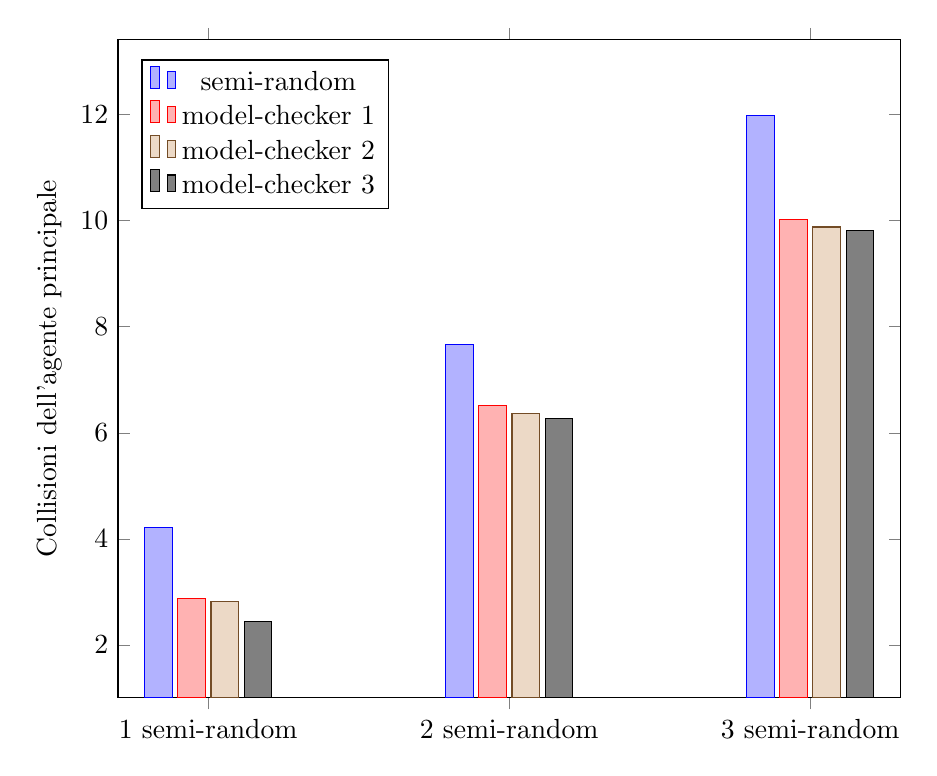
\begin{tikzpicture}[node distance=0.5cm]
	\begin{axis}[
		enlargelimits=0.15,
		width=0.95*\textwidth,
		ybar,
		ylabel=Collisioni dell'agente principale,
		symbolic x coords={1 semi-random,2 semi-random, 3 semi-random},
		xtick=data,
		legend pos= north west
	]
	\addplot coordinates {(1 semi-random,4.22) (2 semi-random,7.67) (3 semi-random,11.98)};
	\addplot coordinates {(1 semi-random,2.87) (2 semi-random,6.52) (3 semi-random,10.02)};
	\addplot coordinates {(1 semi-random,2.82) (2 semi-random,6.36) (3 semi-random,9.88)};
	\addplot coordinates {(1 semi-random,2.44) (2 semi-random,6.27) (3 semi-random,9.82)};
    \legend{semi-random,model-checker 1,model-checker 2,model-checker 3}
	\end{axis}
	\end{tikzpicture}	
		\caption{Grafico dei risultati delle simulazioni: sull'ascissa variano gli agenti che sono realmente nell'area assieme all'agente principale, sull'ordinata viene indicato il numero di collisioni e i diversi colori rappresentano di diversi scheduler utilizzati dall'agente principale.}
	\label{fig:sim_results}
\end{figure}

In tabella \ref{tab:sim_results} vengono riportate le medie dei test effettuati, raffigurate nel grafico \ref{fig:sim_results}. Dal grafico si riesce ad osservare un effettivo miglioramento del risultato dello scheduler basato sul model-checker rispetto a quello semi-casuale. Si percepisce, seppure in minor misura, un leggero miglioramento all'aumentare della complessità dello scenario ipotizzato: anche nel caso in cui le simulazioni prevedano solamente un agente secondario si riscontra una media di collisioni per test più bassa se la \texttt{Hashtable} viene generata su ipotesi più complesse, assumendo due o tre agenti secondari. Nello scenario reale che comprende due agenti esterni si verifica un leggero miglioramento medio passando dallo scheduler generato sull'ipotesi di un solo agente semi-casuale a quello che ne considera due: questo miglioramento è giustificato dal fatto che gli stati previsti sono un numero maggiore e se lo scheduler basato sul model-checker non dovesse trovare lo stato che sta cercando all'interno della \texttt{Hashtable} allora si comporterà come uno scheduler semi-casuale.
% TODO un algoritmo ad hoc sarebbe stato comunque migliore

Le simulazioni tra agenti che utilizzano solo scheduler basati su model-checker danno origine a fenomeni che rendono i risultati non confrontabili con quelli mostrati finora. Tendono a crearsi situazioni ottime e pessime a seconda dei casi: in alcune occasioni tutti gli agenti si stabilizzano in una posizione di equilibrio dove nessuno ha interesse nello spostarsi, in altre lo scenario si ripete con un periodo più ampio portando a oscillazioni tra più zone ma ripetendo gli stessi errori dovuti all'approccio deterministico dello scheduler. Nel caso positivo si ha un numero di collisioni quasi sempre nullo mentre in quello negativo ci si avvicina al $50\%$ della lunghezza della simulazione per il fenomeno sopra descritto. Questo comportamento è giustificato dal fatto che tutti gli agenti hanno lo stesso comportamento deterministico e quindi ricercano le stesse condizioni. Si osserva quindi una situazione di equilibrio instabile che dipende dallo stato iniziale della situazione: se un agente incorre in un caso di collisioni cicliche sarà impossibile uscirne.